\section{Úloha~č.~1}
\subsection{Zadanie}
Stanovte napětí $U_{R3}$ a proud $I_{R3}$. Použijte metodu postupného zjednodušování obvodu.
\begin{table}[H]
\begin{center}
  \begin{tabular}{|c|c|c|c|c|c|c|c|c|c|}
    \hline
    sk. & $U [V]$ & $R_{1} [\Omega]$ & $R_{2} [\Omega]$ 
    &  $R_{3} [\Omega]$ &  $R_{4} [\Omega]$ &  $R_{5} [\Omega]$
    &  $R_{6} [\Omega]$ &  $R_{7} [\Omega]$ &  $R_{8} [\Omega]$ \\ 
    \hline
    F & 125 & 510 & 500 & 550 & 250 & 300 & 800 & 330 & 250 \\ 
    \hline
  \end{tabular}
\end{center}
\end{table}
\begin{center}
  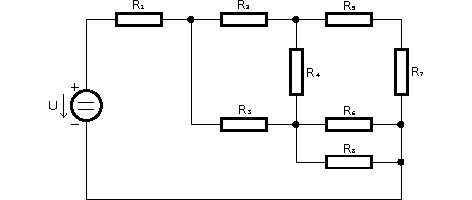
\includegraphics[width=0.8\columnwidth,keepaspectratio]{res/u1o1}
\end{center}
\subsection{Riešenie}
Prevedieme rezistory $R_{2}, R_{3}, R_{4}$ z trojuholníka na hviezdu:
\begin{center}
  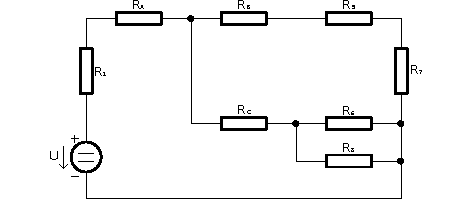
\includegraphics[width=0.8\columnwidth,keepaspectratio]{res/u1o2}
\end{center}
\begin{align*}
    R_{A} &= \frac{R_{2}.R_{3}}{R_{2} + R_{3} + R_{4}} = \frac{500.550}{500 +
550 + 250} = 211,53846~\Omega \\
R_{B} &= \frac{R_{2}.R_{4}}{R_{2} + R_{3} + R_{4}} = \frac{500.250}{500 +
550 + 250} = 96,153846~\Omega \\
R_{C} &= \frac{R_{3}.R_{4}}{R_{2} + R_{3} + R_{4}} = \frac{550.250}{500 +
550 + 250} = 105,76923~\Omega 
\end{align*}
Vypočítame rezistory $R_{1}$ a $R_{A}$ v sérií, ďalej $R_{B}$, $R_{5}$ a $R_{7}$ tiež v sérií, a $R_{6}$ a $R_{8}$ paralelne:
\begin{center}
  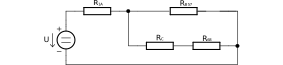
\includegraphics[width=0.8\columnwidth,keepaspectratio]{res/u1o3}
\end{center}
\begin{align*}
    &R_{1A} = R_{1} + R_{A} = 510 + 211,53846 = 721,53846~\Omega \\
    &R_{B57} = R_{B} + R_{5} + R_{7} = 96,153846 + 300 + 330 =
726,153846~\Omega \\
&R_{68} = \frac{R_{6}.R_{8}}{R_{6} + R_{8}} = \frac{800.250}{800 + 250} =
190,47619~\Omega \\
\end{align*}
Vypočítame rezistory $R_{C}$ a $R_{68}$ v sérií:
\begin{center}
  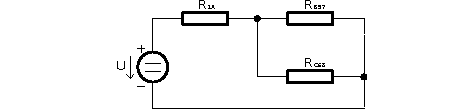
\includegraphics[width=0.8\columnwidth,keepaspectratio]{res/u1o4}
\end{center}
\begin{align*}
    R_{C68} &= R_{C} + R_{68} = 105,76923 + 190,47619 = 296,24542~\Omega \\
\end{align*}
Vypočítame rezistory $R_{B57}$ a $R_{C68}$ paralelne:
\begin{center}
  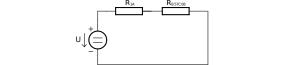
\includegraphics[width=0.8\columnwidth,keepaspectratio]{res/u1o5}
\end{center}
\begin{align*}
    R_{B57C68} &= \frac{R_{B57}.R_{C68}}{R_{B57} + R_{C68}} =
        \frac{726,153846.296,24542}{726,153846 + 296,24542} = 210,40679~\Omega \\
\end{align*}
Vypočítame si výsledný odpor obvodu $R_{EKV}$:
\begin{center}
  
\includegraphics[width=0.8\columnwidth,keepaspectratio]{res/u1o6}
\end{center}
\begin{align*}
    &R_{EKV} = R_{1A} + R_{B57C68} = 721,53846 + 210,40679 = 931,94525~\Omega
\end{align*}
Z odporu $R_{EKV}$ vypočítame prúd $I$ tečúci obvodom:
\begin{align*}
    &I = \frac{U}{R_{EKV}} = \frac{125}{931,94525} = 0,13413~A
\end{align*}
\newpage
V obvode si vytvoríme slučku, aby sme mohli vypočítať napätie $U_{R3}$:
\begin{center}
  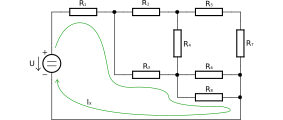
\includegraphics[width=0.8\columnwidth,keepaspectratio]{res/u1o7}
\end{center}
Napíšeme si pre slučku $I_{X}$ rovnicu:
\begin{align*}
    &I_{X}: U_{R1} + U_{R3} + U_{R8} - U = 0 
\end{align*}
Aby sme mohli vypočítať $U_{R3}$, potrebujeme poznať aj $U_{R1}$ a $U_{R8}$. Prvé vypočítame $U_{R1}$:
\begin{align*}
&U_{R1} = R_{1} I = 510 . 0,13413 = 68,4063~V 
\end{align*}
Druhé vypočítame $U_{R8}$:
\begin{align*}
&U_{RB57C68} = R_{B57C68}.I = 210,40679 . 0,13413 = 28,221862743~V \\
&I_{RC68} = \frac{U_{RB57C68}}{R_{C68}} = \frac{28,221862743}{296,24542} = 0,095265144~A \\
&U_{R68} = R_{68}.I_{RC68} = 190,47619.0,095265144 = 18,145741669~V \\
&U_{R8} = U_{R68}  = 190,47619.0,095265144 = 18,145741669~V 
\end{align*}
Dosadíme hodnoty do rovnice a vypočítame $U_{R3}$: 
\begin{align*} &I_{X}: U_{R1} + U_{R3} + U_{R8} - U = 0 \\
&I_{X}: U_{R3} = U - U_{R1} - U_{R8} \\
&I_{X}: U_{R3} = 125 - 68,4063 - 18,145741669 = 38,4480~V 
\end{align*}
Posledné vypočítame $I_{R3}$:
\begin{align*}
&I_{R3} = \frac{U_{R3}}{R_{3}} = \frac{38,447958331}{550} = 0,0699~A
\end{align*}
\newpage
